% =============================================================================
% 4 Entwicklung und Vorauswahl der Stellkonzepte
% =============================================================================
\begingroup
\setlength{\emergencystretch}{0.75em}

\section{Entwicklung und Vorauswahl der Stellkonzepte}
\label{chap:entwicklung_stellkonzept}
\label{chap:konzeptentwicklung}

Die Analyse des bestehenden Erwärmungsprüfstands hat gezeigt, dass die
zentrale Regelung des Gesamtstroms keine automatische Einhaltung der
einzelnen Modulströme gewährleistet. Ursache hierfür sind die unterschiedliche
Impedanz der parallel gespeisten Abgänge, die thermische Änderung der
V2A-Lastwiderstände und die gemeinsame Speisespannung. Aus diesen
Zusammenhängen wurden in Abschnitt~\ref{sec:anforderungen_optimierung} die
Anforderungen an ein automatisiertes Stellkonzept abgeleitet.

Ziel dieses Kapitels ist die Entwicklung und technische Vorauswahl geeigneter
Wirkprinzipien. Untersucht werden vier Ansätze, die an unterschiedlichen
Stellen des Prüfstromkreises ansetzen. Bei den ersten beiden Konzepten wird
parallel zum vorhandenen V2A-Lastwiderstand ein zusätzlicher ohmscher
beziehungsweise induktiver Strompfad vorgesehen. Die beiden weiteren
Konzepte verwenden einen zusätzlichen Transformator, im Folgenden als
Trafo~2 bezeichnet, und einen motorisch verstellbaren Widerstand. Sie
unterscheiden sich darin, ob diese Anordnung auch im
\SI{630}{\ampere}-Abgang eingesetzt wird oder ob der größte Abgang unmittelbar
über den vorhandenen Säulenstelltransformator geregelt wird.

Die Konzeptbewertung erfolgt in zwei Stufen. Zunächst werden Wirkprinzip,
Stellrichtung und grundsätzliche Realisierbarkeit untersucht. Ein Konzept wird
nicht weiterverfolgt, wenn bereits auf dieser Ebene ein wesentliches
Ausschluss\-kriterium vorliegt, beispielsweise eine ungeeignete Kontaktierung im
Hochstrom\-kreis oder ein nicht vertretbarer Bauraum. Konzepte ohne ein solches
Ausschluss\-kriterium werden für die spätere Modellierung und Simulation
vorausgewählt. Die Vorauswahl stellt daher noch keine endgültige
Dimensionierung oder Entscheidung für die praktische Umsetzung dar.


% -----------------------------------------------------------------------------
% 4.1 Randbedingungen und Bewertungsmaßstab
% -----------------------------------------------------------------------------
\subsection{Randbedingungen und Bewertungsmaßstab}
\label{sec:randbedingungen_bewertung_stellkonzepte}

Die Stellkonzepte müssen die in Kapitel~\ref{chap:analyse_pruefstand}
beschriebene Belastungs\-konfiguration mit Abgangs\-strömen zwischen
\SI{40}{\ampere} und \SI{630}{\ampere} abdecken. Dabei ist zwischen dem
Strom eines vollständigen Abgangs und den phasenbezogenen Regelkanälen zu
unterscheiden. Für zwölf dreiphasige Abgänge stehen 36 Modulstrommesswerte zur
Verfügung. Ob die drei Außenleiter eines Abgangs mechanisch gemeinsam oder
unabhängig gestellt werden können, hängt von den verbleibenden
Phasen\-abweichungen ab. Ein Konzept muss daher grundsätzlich eine
phasen\-selektive Ausführung ermöglichen, auch wenn eine spätere Untersuchung
für einzelne Stromklassen eine mechanische Kopplung zulässt.

Für die Konzeptentwicklung wird ein Außenleiter eines Abgangs betrachtet. Die
zugehörigen Größen sind als komplexe Effektivwertzeiger zu verstehen. Der
Strom des Abgangs setzt sich aus dem Strom durch den vorhandenen
V2A-Lastpfad und dem Strom eines zusätzlichen Stellpfads zusammen:

\begin{equation}
    \underline{I}_{k}
    =
    \underline{I}_{\mathrm{V2A},k}
    +
    \underline{I}_{\mathrm{St},k}.
    \label{eq:konzept_stromsumme}
\end{equation}

Für den Betrag des Modulstroms muss

\begin{equation}
    \left|\underline{I}_{k}\right|
    =
    I_{\mathrm{soll},k}
    \label{eq:konzept_sollstrombedingung}
\end{equation}

gelten. Gleichung~\ref{eq:konzept_stromsumme} ist bewusst als Zeigergleichung
formuliert. Bei einem ohmschen Zusatzpfad sind die Teilströme näherungsweise
phasengleich. Bei einem induktiven oder transformatorgekoppelten Stellpfad
müssen dagegen Betrag und Phasenlage berücksichtigt werden. Eine rein
arithmetische Addition der Strombeträge wäre in diesen Fällen nicht zulässig.

In allen Konzepten bleiben die vorhandenen V2A-Widerstände als Grundimpedanz
bestehen. Der zusätzliche Stellpfad soll die
temperatur\-bedingte Änderung des V2A-Stroms ausgleichen und nicht den gesamten
Prüfstrom übernehmen. Dadurch kann der erforderliche Stell\-bereich gegenüber
einem vollständigen Ersatz der bestehenden Last\-widerstände reduziert werden.
Gleichzeitig folgt daraus eine wichtige Rand\-bedingung: Ein parallel
geschalteter passiver Stellpfad kann dem Abgang grundsätzlich nur zusätz\-lichen
Strom zuführen. Der durch den V2A-Pfad allein verursachte Strom darf daher im
gesamten vorgesehenen Arbeits\-bereich nicht oberhalb des Sollstroms liegen.
Der V2A-Widerstand ist im Ausgangs\-zustand so einzustellen, dass eine
ausreichende positive Stell\-reserve verbleibt.

Die gemeinsame Einspeisung koppelt die Regelkanäle weiterhin miteinander.
Ändert ein Stellpfad den Abgangsstrom, ändern sich der Gesamtstrom und damit
die Spannungsabfälle an den gemeinsamen Einspeiseimpedanzen. Umgekehrt wirkt
eine Veränderung der Stellung des Säulenstelltransformators auf sämtliche
Abgänge. Ein lokales Stellglied beseitigt diese Kopplung somit nicht
vollständig, ermöglicht jedoch eine gezielte Korrektur der Stromverteilung.
Das Zusammenwirken zentraler und lokaler Stellgrößen bildet deshalb ein
wesentliches Bewertungskriterium.

Neben der erreichbaren Stromänderung sind die sehr niedrige Prüfspannung und
die hohen Ströme maßgebend. Ein geringer Spannungsabfall an einem Kontakt oder
Leistungshalbleiter beansprucht bereits einen erheblichen Anteil der
verfügbaren Spannung. Bewegte Kontakte im Primärkreis sind wegen ihrer
Verlustleistung und des Risikos kurzzeitiger Stromunterbrechungen besonders
kritisch. Thermisch wirksame Zusatzkomponenten sollen nach Möglichkeit
außerhalb des für den Prüfling maßgebenden Temperaturfelds angeordnet werden.

Für die Vorauswahl werden die in Tabelle~\ref{tab:anforderungen_optimierung}
festgelegten Anforderungen zu fünf Bewertungsgruppen zusammengefasst:

\begin{itemize}
    \item elektrische Stellwirkung und ausreichende Stellreserve,
    \item hochstromtaugliche und dauerbetriebsfeste Ausführung,
    \item Automatisierbarkeit und Einbindung in die vorhandene Mess- und
          Steuerungstechnik,
    \item Beherrschung der Kopplung zwischen den Abgängen sowie
    \item konstruktive Realisierbarkeit und Skalierbarkeit auf den
          vollständigen Prüfstand.
\end{itemize}

Eine quantitative Nutzwertanalyse wird an dieser Stelle nicht durchgeführt.
Für die beiden zunächst weiterzuverfolgenden Konzepte fehlen vor der
Modellbildung belastbare Angaben zu Stellbereich, Regeldynamik und
Verlustleistung. Eine numerische Gewichtung würde daher eine Genauigkeit
vortäuschen, die durch den gegenwärtigen Entwicklungsstand nicht begründet
ist. Die Vorauswahl erfolgt stattdessen anhand nachvollziehbarer technischer
Ausschluss- und Eignungskriterien.


% -----------------------------------------------------------------------------
% 4.2 Paralleler motorisch verstellbarer V2A-Widerstand
% -----------------------------------------------------------------------------
\subsection{Paralleler motorisch verstellbarer V2A-Widerstand}
\label{sec:konzept_paralleler_v2a}

Der erste Ansatz ergänzt den vorhandenen V2A-Lastwiderstand um einen zweiten
ohmschen Pfad. Dieser besteht ebenfalls aus einer V2A-Schiene, deren wirksame
Länge durch einen motorisch bewegten Stromabnehmer verändert wird. Beide
Widerstände liegen parallel zwischen dem Ausgang des MCC-Abgangs und dem
Laststernpunkt. Abbildung~\ref{fig:konzept_paralleler_v2a} zeigt das
Wirkprinzip für einen Außenleiter.

\begin{figure}[H]
    \centering
    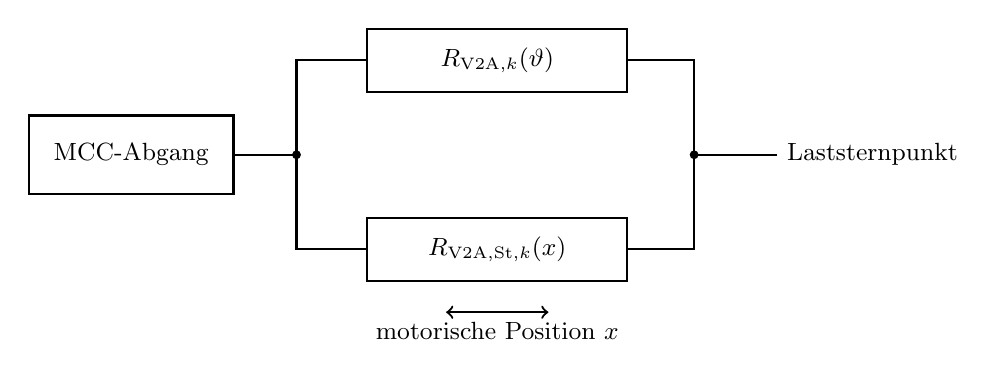
\begin{tikzpicture}[font=\small, line width=0.8pt]
        \node[draw, minimum width=2.6cm, minimum height=1.0cm]
        (mcc) at (0,0) {MCC-Abgang};
        \draw (1.3,0) -- (2.1,0);
        \fill (2.1,0) circle (1.6pt);
        \draw (2.1,0) -- (2.1,1.2) -- (3.0,1.2);
        \draw (2.1,0) -- (2.1,-1.2) -- (3.0,-1.2);
        \node[draw, minimum width=3.3cm, minimum height=0.8cm]
        (v2a) at (4.65,1.2) {$R_{\mathrm{V2A},k}(\vartheta)$};
        \node[draw, minimum width=3.3cm, minimum height=0.8cm]
        (stell) at (4.65,-1.2) {$R_{\mathrm{V2A,St},k}(x)$};
        \draw (6.3,1.2) -- (7.15,1.2) -- (7.15,0);
        \draw (6.3,-1.2) -- (7.15,-1.2) -- (7.15,0);
        \fill (7.15,0) circle (1.6pt);
        \draw (7.15,0) -- (8.2,0);
        \node[anchor=west] at (8.2,0) {Laststernpunkt};
        \draw[<->] (4.0,-2.0) -- node[below] {motorische Position $x$} (5.3,-2.0);
    \end{tikzpicture}
    \caption{Wirkprinzip eines zusätzlichen motorisch verstellbaren
    V2A-Widerstandspfads}
    \label{fig:konzept_paralleler_v2a}
\end{figure}

Werden Leitungs- und Kontaktimpedanzen für die prinzipielle Betrachtung
zunächst vernachlässigt, ergibt sich der Ersatzwiderstand zu

\begin{equation}
    R_{\mathrm{ers},k}
    =
    \left(
        \frac{1}{R_{\mathrm{V2A},k}}
        +
        \frac{1}{R_{\mathrm{V2A,St},k}}
    \right)^{-1}.
    \label{eq:paralleler_v2a_ersatzwiderstand}
\end{equation}

Der resultierende Abgangsstrom lautet bei der Klemmenspannung
$U_k$

\begin{equation}
    I_k
    =
    U_k
    \left(
        \frac{1}{R_{\mathrm{V2A},k}}
        +
        \frac{1}{R_{\mathrm{V2A,St},k}}
    \right).
    \label{eq:paralleler_v2a_strom}
\end{equation}

Erwärmt sich der vorhandene V2A-Widerstand, steigt
$R_{\mathrm{V2A},k}$ und sein Teilstrom sinkt. Durch eine Verringerung der
wirksamen Länge beziehungsweise des Widerstands
$R_{\mathrm{V2A,St},k}$ kann der Strom des Zusatzpfads erhöht und der
Gesamtstrom nachgeführt werden. Das Konzept besitzt damit eine eindeutige,
stetige Stellrichtung. Da beide Pfade näherungsweise ohmsch sind, ist die
Stromaddition im Unterschied zum induktiven Konzept weitgehend phasengleich.

Ein Vorteil dieses Ansatzes ist die unmittelbare Übertragbarkeit des im
bestehenden Prüfstand verwendeten Widerstandsprinzips. Es wird weder ein
zusätzlicher Transformator noch eine leistungselektronische Stromstellung
benötigt. Auch die Verlustleistung und der erforderliche Widerstandswert
lassen sich mit den in Abschnitt~\ref{sec:verlustleistung_temperaturkoeffizient}
beschriebenen Beziehungen bestimmen. Die motorische Position könnte über
einen Spindelantrieb erfasst und durch die vorhandene SPS angesteuert werden.

Das entscheidende Problem liegt jedoch in der bewegten elektrischen
Kontaktierung. Der Stromabnehmer des Zusatzpfads muss während der Verstellung
einen hohen Kompensationsstrom führen. Bereits ein kleiner, zeitlich
veränderlicher Kontaktwiderstand $R_{\mathrm K}$ verursacht die
Verlustleistung

\begin{equation}
    P_{\mathrm K}
    =
    I_{\mathrm{St},k}^{2}R_{\mathrm K}.
    \label{eq:konzept_v2a_kontaktverlust}
\end{equation}

Der quadratische Einfluss des Stroms führt insbesondere in den Abgängen mit
\SI{250}{\ampere}, \SI{400}{\ampere} und \SI{630}{\ampere} zu einer hohen
lokalen thermischen Beanspruchung. Gleichzeitig liegt der Kontaktwiderstand
in derselben Größenordnung wie ein für die Stromaufteilung wirksamer Anteil
der Lastimpedanz. Verschleiß, Verschmutzung oder eine veränderte Anpresskraft
würden damit nicht nur die Erwärmung des Kontakts, sondern unmittelbar auch
die Stellkennlinie beeinflussen.

Während einer Stellbewegung können kurzzeitige Kontakt\-unterbrechungen oder
eine Verringerung der wirksamen Kontaktfläche auftreten. Im bestromten
Hochstrom\-kreis besteht dadurch die Gefahr von Lichtbogen\-bildung und
Kontaktabbrand. Eine sichere Ausführung würde einen speziell für den
Dauerstrom, die Stellbewegung und die geringe Betriebsspannung ausgelegten
Stromabnehmer erfordern. Im Rahmen der Konzeptuntersuchung konnte für die
hohen erforderlichen Teilströme keine geeignete, konstruktiv und thermisch
belastbare Stromabnehmer\-lösung identifiziert werden.

Hinzu kommt, dass der zusätzliche V2A-Pfad selbst erhebliche Verlustwärme
erzeugt. Für jeden Abgang wären Widerstandsschienen, Antrieb, Führung,
Kontaktierung und Berührungsschutz vorzusehen. Die Vervielfachung auf die
erforderlichen Stellkanäle würde den Bauraum und den Wartungsaufwand deutlich
erhöhen. Das Konzept erfüllt zwar grundsätzlich die Anforderungen an eine
stetige Stellwirkung und Automatisierbarkeit, scheitert jedoch an der
hochstromtauglichen Kontaktierung sowie an der thermischen und konstruktiven
Skalierbarkeit. Es wird deshalb nicht weiterverfolgt.


% -----------------------------------------------------------------------------
% 4.3 Induktiver Parallelzweig mit veränderlichem E-I-Kern
% -----------------------------------------------------------------------------
\subsection{Induktiver Parallelzweig mit veränderlichem E-I-Kern}
\label{sec:konzept_ei_kern}

Das zweite Konzept ersetzt den zusätzlichen ohmschen Stellpfad durch eine
veränderliche Drossel. Eine Wicklung befindet sich auf dem Mittelschenkel
eines E-Kerns. Das gegenüberliegende I-Joch wird motorisch verfahren, sodass
sich der Luftspalt $\delta$ und damit die Induktivität verändern. Der
induktive Pfad liegt parallel zum vorhandenen V2A-Lastwiderstand. Die
mechanische Verstellung erfolgt außerhalb des elektrischen Stromübergangs;
ein bewegter Hochstromkontakt wird daher vermieden.

\begin{figure}[H]
    \centering
    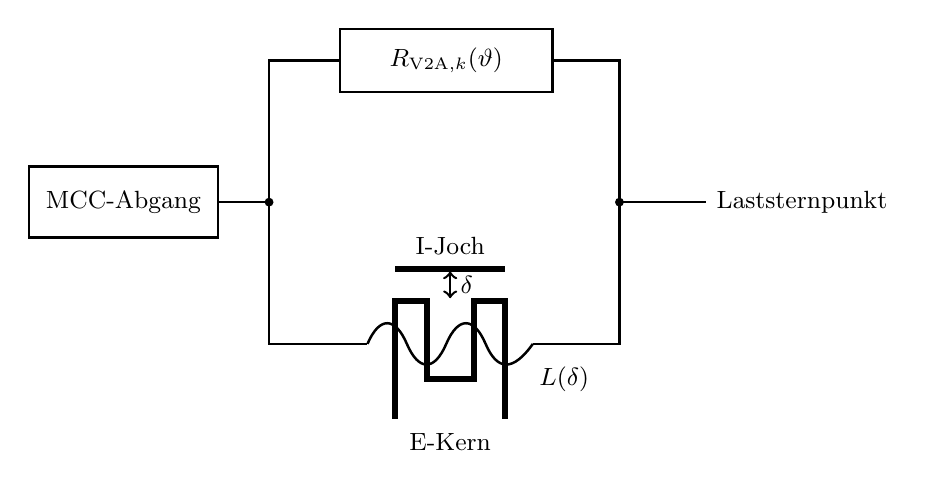
\begin{tikzpicture}[font=\small, line width=0.9pt]
        \node[draw, minimum width=2.4cm, minimum height=0.9cm]
        (mcc) at (-4.3,0) {MCC-Abgang};
        \draw (-3.1,0) -- (-2.45,0);
        \fill (-2.45,0) circle (1.6pt);
        \draw (-2.45,0) -- (-2.45,1.8) -- (-1.55,1.8);
        \node[draw, minimum width=2.7cm, minimum height=0.8cm]
        at (-0.2,1.8) {$R_{\mathrm{V2A},k}(\vartheta)$};
        \draw (1.15,1.8) -- (2.0,1.8) -- (2.0,0);
        \draw (-2.45,0) -- (-2.45,-1.8) -- (-1.2,-1.8);
        \draw (-1.2,-1.8)
        .. controls (-1.05,-1.45) and (-0.85,-1.45) .. (-0.7,-1.8)
        .. controls (-0.55,-2.15) and (-0.35,-2.15) .. (-0.2,-1.8)
        .. controls (-0.05,-1.45) and (0.15,-1.45) .. (0.3,-1.8)
        .. controls (0.45,-2.15) and (0.65,-2.15) .. (0.9,-1.8);
        \draw (0.9,-1.8) -- (2.0,-1.8) -- (2.0,0);
        \fill (2.0,0) circle (1.6pt);
        \draw (2.0,0) -- (3.1,0);
        \node[anchor=west] at (3.1,0) {Laststernpunkt};

        \draw[line width=2.2pt] (-0.85,-2.75) -- (-0.85,-1.25)
        -- (-0.45,-1.25) -- (-0.45,-2.25)
        -- (0.15,-2.25) -- (0.15,-1.25)
        -- (0.55,-1.25) -- (0.55,-2.75);
        \draw[line width=2.2pt] (-0.85,-0.85) -- (0.55,-0.85);
        \draw[<->] (-0.15,-1.22) -- node[right] {$\delta$} (-0.15,-0.88);
        \node at (-0.15,-3.05) {E-Kern};
        \node at (-0.15,-0.55) {I-Joch};
        \node[anchor=west] at (0.85,-2.25) {$L(\delta)$};
    \end{tikzpicture}
    \caption{Wirkprinzip eines induktiven Parallelzweigs mit veränderlichem
    E-I-Kern}
    \label{fig:konzept_ei_kern}
\end{figure}

Die Impedanz des realen Drosselzweigs wird durch den Wicklungswiderstand
$R_{\mathrm{Cu}}$ und die luftspaltabhängige Reaktanz beschrieben:

\begin{equation}
    \underline Z_L(\delta)
    =
    R_{\mathrm{Cu}}
    +
    \mathrm{j}\omega L(\delta).
    \label{eq:ei_impedanz}
\end{equation}

Im linearen magnetischen Bereich gilt nach
Gleichung~\ref{eq:induktivitaet_magnetischer_kreis}

\begin{equation}
    L(\delta)
    =
    \frac{N^2}{\mathcal R_{\mathrm{m,ges}}(\delta)}.
    \label{eq:ei_induktivitaet}
\end{equation}

Mit zunehmendem Luftspalt steigt der magnetische Widerstand. Dadurch sinken
die Induktivität und der induktive Blindwiderstand, während der Strom des
Zusatzpfads zunimmt. Wird der Wicklungswiderstand für die Erklärung des
Wirkprinzips vernachlässigt, ergibt sich

\begin{equation}
    I_L(\delta)
    \approx
    \frac{U_k}{\omega L(\delta)}.
    \label{eq:ei_blindstrom}
\end{equation}

Der V2A-Strom und der ideale induktive Strom sind um annähernd
$90^{\circ}$ gegeneinander phasenverschoben. Der Betrag des Modulstroms ist
daher näherungsweise

\begin{equation}
    I_k
    \approx
    \sqrt{I_{\mathrm{V2A},k}^{2}+I_L^{2}}.
    \label{eq:ei_modulstrombetrag}
\end{equation}

Die Strombelastung des MCC-Abgangs kann somit erhöht werden, ohne die
zusätzliche Leistung vollständig in einem ohmschen Stellwiderstand
umzusetzen. Die Quelle und die gemeinsame Einspeisung müssen jedoch neben der
Wirkleistung des V2A-Pfads die zusätzliche Blindleistung bereitstellen. Die
erforderliche Scheinleistung und die Belastung von Leitungen und
Transformatoren werden deshalb durch den induktiven Pfad nicht vermieden.

Zur Prüfung des Wirkprinzips wurde ein vorhandener E-I-Kern mit einer
Wicklung versehen. Das I-Joch wurde über Distanzstücke auf Luftspalte von
\SI{2}{\milli\metre}, \SI{4}{\milli\metre} und
\SI{10}{\milli\metre} eingestellt. Für jeden Arbeitspunkt wurden die
Strangspannung und die Blindleistung erfasst. Aus den Messwerten wurden der
induktive Strom und die Induktivität mit

\begin{equation}
    I_L
    =
    \frac{Q}{U_{\mathrm{RMS}}},
    \qquad
    L
    =
    \frac{U_{\mathrm{RMS}}^2}{\omega Q}
    \label{eq:ei_versuchsauswertung}
\end{equation}

bestimmt. Gleichung~\ref{eq:ei_versuchsauswertung} setzt für die
Versuchsauswertung einen näherungsweise induktiven Zweig voraus. Die
Messwerte und daraus berechneten Größen sind in
Tabelle~\ref{tab:ei_luftspaltversuch} zusammengefasst.

\begin{table}[H]
    \centering
    \caption{Messwerte des Luftspaltversuchs am vorhandenen E-I-Kern}
    \label{tab:ei_luftspaltversuch}
    \begin{tabular}{ccccc}
        \toprule
        Luftspalt $\delta$ & $U_{\mathrm{RMS}}$ & $Q$ & $I_L$ & $L$ \\
        \midrule
        \SI{2}{\milli\metre}  & \SI{4.3}{\volt} & \(40\,\mathrm{var}\) &
        \SI{9.30}{\ampere} & \SI{1.47}{\milli\henry} \\
        \SI{4}{\milli\metre}  & \SI{4.3}{\volt} & \(54\,\mathrm{var}\) &
        \SI{12.56}{\ampere} & \SI{1.09}{\milli\henry} \\
        \SI{10}{\milli\metre} & \SI{4.3}{\volt} & \(72\,\mathrm{var}\) &
        \SI{16.74}{\ampere} & \SI{0.82}{\milli\henry} \\
        \bottomrule
    \end{tabular}
\end{table}

Der Versuch bestätigt die erwartete Richtung der Stellwirkung. Zwischen
\SI{2}{\milli\metre} und \SI{10}{\milli\metre} sinkt die Induktivität von
etwa \SI{1.47}{\milli\henry} auf \SI{0.82}{\milli\henry}. Gleichzeitig
steigt der induktive Strom von \SI{9.30}{\ampere} auf
\SI{16.74}{\ampere}. Das Wirkprinzip des verfahrbaren I-Jochs ist damit
nachgewiesen. Für die Beurteilung des Stellkonzepts ist jedoch nicht allein
die relative Änderung, sondern vor allem die absolute Stromreserve
entscheidend. Der gesamte Stellhub erzeugte lediglich eine Stromänderung von

\begin{equation}
    \Delta I_L
    =
    \SI{16.74}{\ampere}
    -
    \SI{9.30}{\ampere}
    =
    \SI{7.44}{\ampere}.
    \label{eq:ei_gemessene_stromaenderung}
\end{equation}

Diese Größenordnung reicht insbesondere für die Nachführung der großen
Abgänge nicht aus. Eine einfache Vergrößerung der Windungszahl löst das
Problem nicht. Nach Gleichung~\ref{eq:ei_induktivitaet} geht $N$ quadratisch
in die Induktivität ein. Im luftspalt\-dominierten Bereich kann näherungsweise

\begin{equation}
    I_L(\delta)
    \approx
    \frac{U_k\,\delta}
    {\omega\mu_0N^2A_{\delta}}
    \label{eq:ei_strom_luftspaltnaeherung}
\end{equation}

geschrieben werden. Eine Verringerung der Windungszahl erhöht zwar den
Strompegel quadratisch, erhöht aber sowohl den minimalen als auch den
maximalen Strom des Stellpfads. Das Verhältnis der beiden Grenzströme wird im
linearen Bereich im Wesentlichen durch das Verhältnis der magnetischen
Widerstände und nicht durch $N$ bestimmt. Für einen großen absoluten
Stellbereich bei zugleich kleinem Grundstrom wäre daher eine wesentlich
größere Änderung des magnetischen Widerstands erforderlich.

Bei einer Übertragung auf dreistellige Kompensations\-ströme müssen zudem die
Wicklungs\-leiter entsprechend groß dimensioniert werden. Die Kombination aus
erforderlicher Induktivität, wenigen hochstromfähigen Windungen,
ausreichendem Kern\-querschnitt, erweitertem Luftspalt\-stellweg und den
auftretenden magnetischen Kräften führt zu großen und schweren Komponenten.
Die vorhandenen E-I-Kerne erzeugten im Versuch nicht die erforderliche
Stromänderung. Eine auf den vollständigen Prüfstrombereich skalierte
Ausführung würde den verfügbaren Bauraum und den konstruktiven Aufwand des
Prüfstands unverhältnismäßig erhöhen.

Das Konzept besitzt damit ein physikalisch funktionsfähiges Stellprinzip und
vermeidet einen bewegten elektrischen Hochstromkontakt. Es erfüllt jedoch
nicht die Anforderungen an Stellbereich, Bauraum und Skalierbarkeit. Der
induktive Parallelzweig wird deshalb trotz des erfolgreichen
Wirkungsnachweises nicht weiterverfolgt.


% -----------------------------------------------------------------------------
% 4.4 Trafo 2 und Stellwiderstand in jedem Abgang
% -----------------------------------------------------------------------------
\subsection{Trafo 2 und motorisch verstellbarer Widerstand in jedem Abgang}
\label{sec:konzept_trafo2_alle_abgaenge}

Das dritte Konzept verlagert den bewegten Widerstand aus dem unmittelbaren
Hochstrompfad. Parallel zum vorhandenen V2A-Lastwiderstand wird in jedem
Abgang ein zusätzlicher Transformator angeordnet. An dessen Sekundärseite
befindet sich ein motorisch verstellbarer Widerstand. Über das
Übersetzungsverhältnis von Trafo~2 wird dessen Widerstandsänderung auf die
Primärseite transformiert. Abbildung~\ref{fig:konzept_trafo2_alle} zeigt das
Wirkprinzip für einen phasenbezogenen Stellkanal.

\begin{figure}[H]
    \centering
    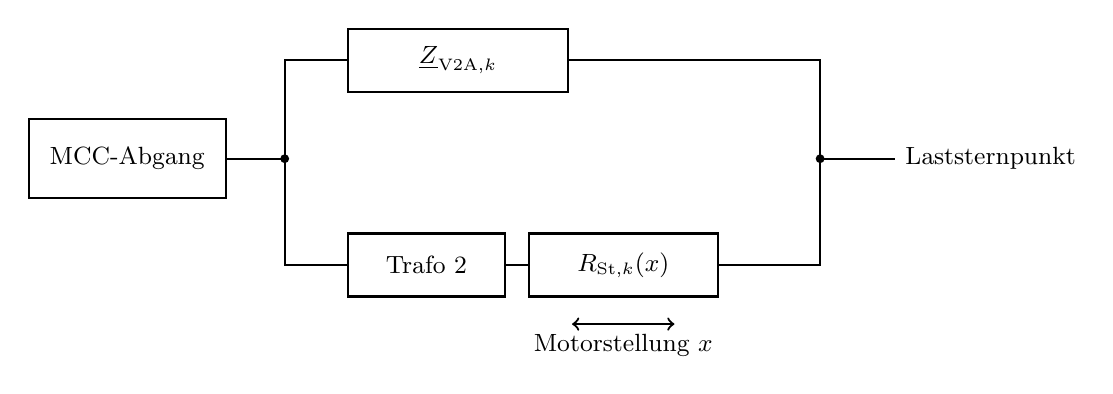
\begin{tikzpicture}[font=\small, line width=0.8pt]
        \node[draw, minimum width=2.5cm, minimum height=1.0cm]
        (mcc) at (0,0) {MCC-Abgang};
        \draw (1.25,0) -- (2.0,0);
        \fill (2.0,0) circle (1.6pt);
        \draw (2.0,0) -- (2.0,1.25) -- (2.8,1.25);
        \node[draw, minimum width=2.8cm, minimum height=0.8cm]
        at (4.2,1.25) {$\underline Z_{\mathrm{V2A},k}$};
        \draw (5.6,1.25) -- (8.8,1.25) -- (8.8,0);

        \draw (2.0,0) -- (2.0,-1.35) -- (2.8,-1.35);
        \node[draw, minimum width=2.0cm, minimum height=0.8cm]
        at (3.8,-1.35) {Trafo~2};
        \draw (4.8,-1.35) -- (5.1,-1.35);
        \node[draw, minimum width=2.4cm, minimum height=0.8cm]
        at (6.3,-1.35) {$R_{\mathrm{St},k}(x)$};
        \draw (7.5,-1.35) -- (8.8,-1.35) -- (8.8,0);
        \fill (8.8,0) circle (1.6pt);
        \draw (8.8,0) -- (9.75,0);
        \node[anchor=west] at (9.75,0) {Laststernpunkt};
        \draw[<->] (5.65,-2.1) -- node[below] {Motorstellung $x$} (6.95,-2.1);
    \end{tikzpicture}
    \caption{Parallelpfad aus Trafo~2 und motorisch verstellbarem
    Sekundärwiderstand}
    \label{fig:konzept_trafo2_alle}
\end{figure}

Für Trafo~2 wird das Übersetzungsverhältnis entsprechend
Gleichung~\ref{eq:transformator_uebersetzung} mit

\begin{equation}
    \ddot{u}_{2}
    =
    \frac{N_1}{N_2}
    =
    \frac{U_1}{U_2}
    =
    \frac{I_2}{I_1}
    \label{eq:konzept_trafo2_uebersetzung}
\end{equation}

definiert. Der sekundärseitige Stellwiderstand erscheint auf der Primärseite
mit

\begin{equation}
    R'_{\mathrm{St},k}
    =
    \ddot{u}_{2}^{\,2}R_{\mathrm{St},k}.
    \label{eq:konzept_trafo2_widerstandstransformation}
\end{equation}

Wird die auf die Primärseite bezogene Kurzschlussimpedanz des Transformators
mit $\underline Z_{\mathrm{k,T2}}$ bezeichnet, kann die Impedanz des
zusätzlichen Pfads in einer vereinfachten Reihendarstellung durch

\begin{equation}
    \underline Z_{\mathrm{St},k}
    =
    \underline Z_{\mathrm{k,T2},k}
    +
    \ddot{u}_{2,k}^{\,2}R_{\mathrm{St},k}
    \label{eq:konzept_trafo2_stellpfadimpedanz}
\end{equation}

beschrieben werden. Der Magnetisierungszweig und die Eisenverluste sind in
dieser Gleichung noch nicht enthalten. Sie werden bei der späteren
Modellierung abhängig von der erforderlichen Modellgüte berücksichtigt. Der
Modulstrom ergibt sich zu

\begin{equation}
    \underline I_k
    =
    \underline U_k
    \left(
        \frac{1}{\underline Z_{\mathrm{V2A},k}}
        +
        \frac{1}{\underline Z_{\mathrm{St},k}}
    \right).
    \label{eq:konzept_trafo2_modulstrom}
\end{equation}

Steigt der V2A-Widerstand infolge der Erwärmung, kann
$R_{\mathrm{St},k}$ verringert und der Strom des transformatorgekoppelten
Parallelpfads erhöht werden. Im Unterschied zum ersten Konzept befindet sich
der bewegte Kontakt nicht im unmittelbaren Niederspannungs-Hochstrom\-kreis.
Wird Trafo~2 sekundärseitig mit einer höheren Spannung betrieben, gilt
$\ddot{u}_{2}<1$ und damit $I_2=\ddot{u}_{2}I_1$. Der Strom durch den
motorisch verstellbaren Widerstand und dessen Kontaktierung ist folglich
kleiner als der auf der Primärseite wirksame Kompensationsstrom. Zugleich
kann ein größerer sekundärseitiger Widerstandswert verwendet werden. Dadurch
werden Kontaktierung, Leiterquerschnitt und mechanische Verstellung technisch
beherrschbarer.

Die Verlustwärme des Stellwiderstands und von Trafo~2 kann räumlich außerhalb
des Prüflings angeordnet werden. Der V2A-Lastwiderstand übernimmt weiterhin
den Grundstrom, während der Transformatorpfad nur die erforderliche
Stellreserve bereitstellt. Damit werden weder der vorhandene Lastaufbau noch
die 50-Hz-Grundfrequenz grundsätzlich verändert. Eine elektrische
Ansteuerung des Antriebs, eine Positionsrückmeldung und die Einbindung in SPS
und WinCC sind mit konventioneller Antriebstechnik möglich.

Die Auslegung von Trafo~2 kann nicht auf das ideale Übersetzungsverhältnis
beschränkt werden. Seine Kurzschlussimpedanz beeinflusst sowohl den
Stellbereich als auch die Phasenlage des Zusatzstroms. Für die spätere
vergleichende Simulation wird als vorläufige Modellannahme eine relative
Kurzschlussspannung von $u_{\mathrm{k}}=\SI{5}{\percent}$ und ein Verhältnis
$X_{\mathrm{k}}/R_{\mathrm{k}}=10$ verwendet. Daraus werden Betrag, Wirk- und
Blindanteil der Kurzschlussimpedanz mit den
Gleichungen~\ref{eq:kurzschlussimpedanz_transformator} und
\ref{eq:rk_xk_transformator} bestimmt. Diese Werte dienen der
Konzeptuntersuchung und ersetzen keine spätere Auslegung anhand realer
Transformator- und Herstellerdaten.

Für den vollständigen Prüfstand entsteht ein erheblicher Komponentenbedarf.
Jeder Abgang benötigt einen geeigneten Trafo~2 und mindestens einen
verstellbaren Widerstand. Soll eine phasenselektive Nachführung umgesetzt
werden, müssen die drei sekundärseitigen Widerstände beziehungsweise ihre
Stellbewegungen unabhängig beeinflussbar sein. Alternativ kann ein
dreiphasiger Transformator mit drei getrennten Stellpfaden verwendet werden.
Die konkrete Bauform ist Bestandteil der späteren konstruktiven Auslegung.

Weitere Nachteile sind die Kupfer- und Eisenverluste der Transformatoren,
der zusätzliche Bauraum und der Wartungsaufwand der motorischen Stellglieder.
Die Regelkanäle bleiben über die gemeinsame Quelle gekoppelt. Deshalb muss
untersucht werden, ob Stellbereich und Regeldynamik auch bei gleichzeitiger
Nachführung mehrerer Abgänge ausreichen. Diese offenen Punkte stellen jedoch
kein unmittelbares Ausschlusskriterium dar. Das Konzept vermeidet die
bewegte Hochstromkontaktierung und ist auf die unterschiedlichen Stromklassen
durch eine angepasste Transformatorübersetzung skalierbar. Es wird daher für
die Modellbildung und Simulation vorausgewählt.


% -----------------------------------------------------------------------------
% 4.5 Regelung des 630-A-Abgangs über den Säulenstelltransformator
% -----------------------------------------------------------------------------
\subsection{Regelung des 630-A-Abgangs über den Säulenstelltransformator}
\label{sec:konzept_saeulentrafo_630}

Das vierte Konzept baut auf der transformatorgestützten Nachführung auf,
verwendet für den größten Abgang jedoch kein zusätzliches lokales
Stellglied. Der vorhandene Säulenstelltransformator wird so geregelt, dass
der Strom des \SI{630}{\ampere}-Abgangs seinem Sollwert folgt. Der
V2A-Lastwiderstand bleibt auch in diesem Abgang als Grundimpedanz erhalten.
Lediglich Trafo~2 und der lokale motorische Stellwiderstand entfallen im
\SI{630}{\ampere}-Pfad. Die übrigen Abgänge erhalten weiterhin jeweils einen
transformatorgekoppelten Stellpfad nach
Abschnitt~\ref{sec:konzept_trafo2_alle_abgaenge}.

\begin{figure}[H]
    \centering
    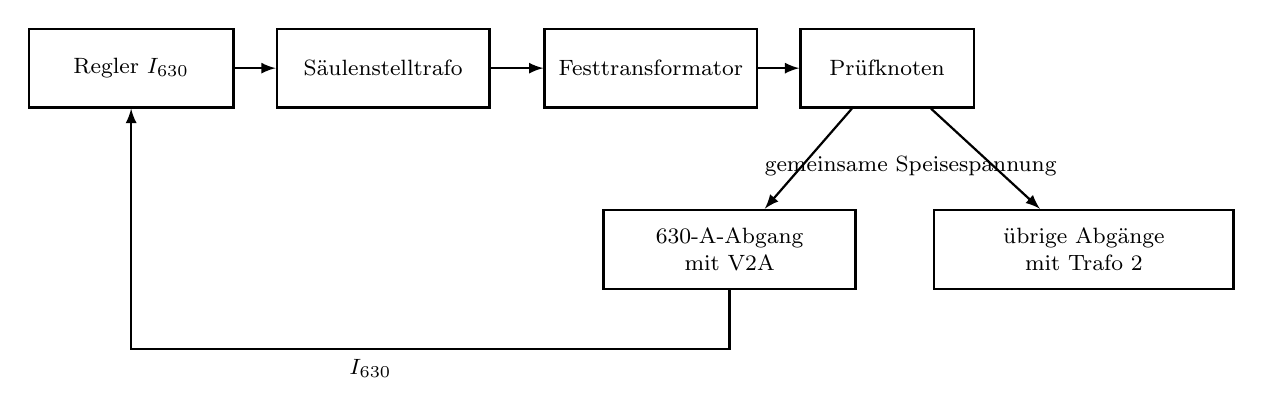
\begin{tikzpicture}[font=\footnotesize, line width=0.8pt, >=latex]
        \node[draw, minimum width=2.6cm, minimum height=1.0cm]
        (reg) at (-5.1,1.6) {Regler $I_{630}$};
        \node[draw, minimum width=2.7cm, minimum height=1.0cm]
        (sst) at (-1.9,1.6) {Säulenstelltrafo};
        \node[draw, minimum width=2.7cm, minimum height=1.0cm]
        (fest) at (1.5,1.6) {Festtransformator};
        \node[draw, minimum width=2.2cm, minimum height=1.0cm]
        (knoten) at (4.5,1.6) {Prüfknoten};
        \draw[->] (reg) -- (sst);
        \draw[->] (sst) -- (fest);
        \draw[->] (fest) -- (knoten);

        \node[draw, align=center, minimum width=3.2cm, minimum height=1.0cm]
        (a630) at (2.5,-0.7) {630-A-Abgang\\mit V2A};
        \node[draw, align=center, minimum width=3.8cm, minimum height=1.0cm]
        (rest) at (7.0,-0.7) {übrige Abgänge\\mit Trafo~2};
        \draw[->] (knoten) -- (a630);
        \draw[->] (knoten) -- (rest);
        \node at (4.8,0.35) {gemeinsame Speisespannung};
        \draw[->] (a630.south) -- ++(0,-0.75) -| node[pos=0.30,below]
        {$I_{630}$} (reg.south);
    \end{tikzpicture}
    \caption{Regelungsstruktur mit dem \SI{630}{\ampere}-Abgang als
    Führungsabgang}
    \label{fig:konzept_saeulentrafo_630}
\end{figure}

Für den Führungsabgang wird die Regeldifferenz phasenbezogen aus

\begin{equation}
    e_{630}(t)
    =
    I_{\mathrm{soll},630}
    -
    I_{630}(t)
    \label{eq:konzept_regelfehler_630}
\end{equation}

gebildet. Die drei motorischen Antriebe des Säulenstelltransformators bilden
die zugehörigen zentralen Stellgrößen. Erwärmt sich der
V2A-Lastwiderstand des \SI{630}{\ampere}-Abgangs, wird die Speisespannung so
weit erhöht, bis der vorgesehene Strom wieder erreicht ist. Der größte
Abgang nutzt damit unmittelbar das bereits vorhandene und für die
Hochstromeinspeisung ausgelegte Stellglied.

Die Spannungsänderung wirkt gleichzeitig auf alle anderen Lastzweige. Deren
lokale Regler müssen sowohl den eigenen thermischen Drift als auch die durch
den Führungsabgang verursachte Spannungsänderung ausgleichen. Für einen
übrigen Abgang $k$ gilt weiterhin

\begin{equation}
    \underline I_k(t)
    =
    \underline I_{\mathrm{V2A},k}(t)
    +
    \underline I_{\mathrm{T2},k}(t),
    \label{eq:konzept_master_slave_strom}
\end{equation}

wobei $\underline I_{\mathrm{T2},k}$ durch den sekundärseitigen
Stellwiderstand beeinflusst wird. Damit der Parallelpfad in beide für die
Nachführung erforderlichen Richtungen wirksam werden kann, muss seine
Ausgangsstellung einen endlichen Zusatzstrom bereitstellen. Eine Erhöhung des
Stellwiderstands reduziert diesen Zusatzstrom, eine Verringerung erhöht ihn.
Der passive V2A-Anteil darf bei der größten vom Säulenstelltransformator
erzeugten Klemmenspannung den jeweiligen Sollstrom nicht überschreiten:

\begin{equation}
    \left|
        \frac{\underline U_{k,\max}}
             {\underline Z_{\mathrm{V2A},k,\min}}
    \right|
    \leq
    I_{\mathrm{soll},k}.
    \label{eq:konzept_630_passivbedingung}
\end{equation}

Ist diese Bedingung verletzt, kann der parallele Transformatorpfad die
Überhöhung nicht kompensieren, da ein passiver Zusatzpfad keinen Strom aus
dem Modulstrom subtrahiert. Die anfängliche Einstellung der
V2A-Last\-widerstände und der verfügbare Widerstandsbereich sind deshalb
gemeinsam mit dem maximalen Spannungsstellbereich auszulegen.

Der wesentliche Vorteil des Konzepts besteht darin, dass die aufwendigste
lokale Anordnung aus Transformator und Stellwiderstand im
\SI{630}{\ampere}-Abgang entfällt. Gerade dort wären Stromtrag\-fähigkeit,
Transformatorleistung und Leiterquerschnitte am größten. Gleichzeitig wird
die thermische Drift des für die Speisespannung maßgebenden Abgangs direkt
durch den vorhandenen Säulenstelltransformator ausgeglichen. Gegenüber dem
dritten Konzept sinken Komponentenbedarf, Bauraum und zusätzliche
Verlustleistung.

Dem steht eine stärkere regelungstechnische Kopplung gegenüber. Der zentrale
Regler und die lokalen Regler dürfen sich nicht durch fortlaufende
gegenläufige Stellbewegungen anregen. Erforderlich sind eine abgestimmte
Dynamik, geeignete Totzonen und gegebenenfalls eine zeitliche Trennung der
Stellvorgänge. Da der thermische Drift langsam verläuft, ist eine solche
Koordination grundsätzlich möglich; ihre Wirksamkeit kann jedoch nicht allein
aus der statischen Konzeptbetrachtung abgeleitet werden.

Weiterhin ist zu untersuchen, ob der Säulenstelltransformator für alle drei
Außenleiter genügend Stellreserve besitzt und ob seine mechanische
Stellgeschwindigkeit für den Führungsregler ausreicht. Ein Mess- oder
Stellfehler im \SI{630}{\ampere}-Kanal würde auf die Speisespannung aller
Abgänge wirken und erfordert daher eine Grenzüberwachung. Diese Punkte sind
für die Regelungs- und Sicherheitsauslegung wesentlich, bilden aber kein
grundsätzliches Ausschlusskriterium. Das Konzept wird deshalb ebenfalls für
die Modellbildung und Simulation vorausgewählt.


% -----------------------------------------------------------------------------
% 4.6 Vergleich und Vorauswahl
% -----------------------------------------------------------------------------
\subsection{Vergleich und Auswahl der weiterzuverfolgenden Konzepte}
\label{sec:vergleich_vorauswahl_stellkonzepte}

Die vier Konzepte greifen auf unterschiedliche Weise in die Stromverteilung
ein. Der parallele V2A-Pfad und der induktive E-I-Kern-Pfad wurden bis zu
einem praktisch entscheidenden Ausschlusskriterium untersucht. Bei den beiden
transformatorgestützten Varianten ist die grundsätzliche technische
Realisierbarkeit gegeben; die noch offenen Fragen betreffen vor allem die
Dimensionierung und das dynamische Zusammenwirken der Regelkanäle.
Tabelle~\ref{tab:vergleich_stellkonzepte} fasst die Vorauswahl zusammen.

\begin{table}[H]
    \centering
    \caption{Qualitativer Vergleich und Vorauswahl der Stellkonzepte}
    \label{tab:vergleich_stellkonzepte}
    \small
    \begin{tabular}{p{0.22\textwidth}p{0.595\textwidth}p{0.095\textwidth}}
        \toprule
        Konzept & Technische Bewertung & Auswahl \\
        \midrule
        Motorischer V2A-Parallelpfad &
        Stetige, näherungsweise phasengleiche Stromstellung; jedoch bewegter
        Hochstromkontakt mit Kontaktverlusten, Lichtbogenrisiko und hohem
        thermischem sowie konstruktivem Aufwand &
        nein \\
        \addlinespace
        E-I-Kern-Parallelzweig &
        Keine bewegte elektrische Kontaktstelle und geringe ohmsche
        Zusatzverluste; die gemessene Stromänderung von nur
        \SI{7.44}{\ampere} ist für große Abgänge unzureichend. Wicklung,
        Kern und Bauraum wären unverhältnismäßig zu vergrößern &
        nein \\
        \addlinespace
        Trafo~2 in jedem Abgang &
        Verlagerung des Stellwiderstands in einen günstigeren Spannungs- und
        Strombereich; an die Stromklassen anpassbar. Komponentenbedarf,
        Transformatorverluste und Kopplung sind noch zu untersuchen &
        ja \\
        \addlinespace
        630-A-Führungsabgang &
        Nutzung des vorhandenen Säulenstelltransformators und Entfall der
        größten lokalen Trafo-2-Anordnung; dafür stärkere Kopplung zwischen
        Führungsabgang und lokalen Regelkanälen &
        ja \\
        \bottomrule
    \end{tabular}
\end{table}

Das erste Konzept wird vor allem durch die Anforderungen A11
``Hochstromtaugliche Kontaktierung'' und A14 ``Skalierbarkeit und Aufwand''
ausgeschlossen. Beim E-I-Kern-Konzept sind die Anforderungen A2
``Strombereich'', A4 ``Stellbereich und Reserve'' sowie A12
``Konstruktive Realisierbarkeit'' mit den vorhandenen Komponenten nicht
erfüllbar. Der Versuch hat die magnetische Stellwirkung bestätigt, zugleich
aber die für den Prüfstand unzureichende absolute Stromänderung belegt.

Die beiden transformatorgestützten Konzepte vermeiden die entscheidenden
Schwachstellen der verworfenen Ansätze. Durch die Impedanztransformation kann
der bewegte Widerstand bei höherer Spannung und geringerem Strom betrieben
werden. Damit wird keine bewegte Kontaktstelle für den unmittelbaren
Hochstrompfad benötigt. Gleichzeitig bleibt der vorhandene V2A-Widerstand als
Grundlast erhalten. Beide Konzepte sind mit motorischen Antrieben,
Positionsrückmeldung und der vorhandenen SPS grundsätzlich automatisierbar.

Eine endgültige Auswahl zwischen den beiden Varianten ist auf Grundlage der
Konzeptbetrachtung noch nicht möglich. Das Konzept mit Trafo~2 in jedem
Abgang besitzt eine gleichartige dezentrale Struktur, erfordert jedoch auch
im \SI{630}{\ampere}-Pfad eine entsprechend leistungsfähige zusätzliche
Anordnung. Das Konzept mit dem \SI{630}{\ampere}-Abgang als Führungsabgang
reduziert den Komponentenbedarf, erhöht aber die regelungstechnische Kopplung.
Für die Entscheidung sind insbesondere folgende Größen zu untersuchen:

\begin{itemize}
    \item erforderlicher primär- und sekundärseitiger Stellbereich,
    \item Einfluss von Übersetzungsverhältnis und Kurzschlussimpedanz von
          Trafo~2,
    \item Stellreserve im kalten und thermisch eingeschwungenen Zustand,
    \item gegenseitige Beeinflussung bei gleichzeitigen Stellvorgängen,
    \item Regeldynamik und Schwingungsneigung sowie
    \item zusätzliche Verlustleistung und Anzahl der benötigten Komponenten.
\end{itemize}

Als Ergebnis der Vorauswahl werden daher das Konzept mit Trafo~2 und
Stellwiderstand in jedem Abgang sowie das Konzept mit zentral geregeltem
\SI{630}{\ampere}-Abgang weiterverfolgt. Die dafür benötigte Modellgrundlage
wird in Kapitel~\ref{chap:modellbildung} zunächst aus dem elektrischen und
thermischen Verhalten des bestehenden Prüfstands abgeleitet. Anschließend
können beide Stellkonzepte unter identischen Randbedingungen simuliert und
miteinander verglichen werden.

\endgroup